\documentclass[10pt,twocolumn,letterpaper]{article}

\usepackage{cvpr}
\usepackage{times}
\usepackage{epsfig}
\usepackage{graphicx}
\usepackage{amsmath}
\usepackage{amssymb}

% Include other packages here, before hyperref.

% If you comment hyperref and then uncomment it, you should delete
% egpaper.aux before re-running latex.  (Or just hit 'q' on the first latex
% run, let it finish, and you should be clear).
\usepackage[breaklinks=true,bookmarks=false]{hyperref}

\cvprfinalcopy % *** Uncomment this line for the final submission

% Pages are numbered in submission mode, and unnumbered in camera-ready
%\ifcvprfinal\pagestyle{empty}\fi
\setcounter{page}{1}
\begin{document}

%%%%%%%%% TITLE
\title{Implementation of Deep High-Resolution Representation\\ Learning for Visual Recognition}

\author{Shiyao Xie\\
2016xxxxxx\\
\and
Zeyuan Yang\\
2017011577\\
\and
Zifei Zhu\\
2017xxxxxx\\
\and
Shengge Yang\\
2016xxxxxx\\
}

\maketitle
%\thispagestyle{empty}

%%%%%%%%% ABSTRACT
\begin{abstract}
   High-Resolution representation is a popular topic in computer vision research field.
   After researching on related works in this field,
   we decided to implement a recent released paper at IEEE 2020,
   \emph{Deep High-Resolution Representation Learning for Visual Recognition} (HRnet).\cite{wang2019deep}
   To completely comprehend the paper,
   we reproduced the code and ran it on an open source dataset.
   Moreover, the structure and outputs are compared with the source code.
\end{abstract}

%%%%%%%%% BODY TEXT
\section{Introduction}

In many fields, high-resolution representation is important,
such as human position detecting.
How to extract key features from high-resolution images becomes a popular topic,
also a challenging problem.
Almost all previous state-of-art works share a similar method,
which is applying a high-to-low resolution network and extracting high-resolution representation from low-resolution features.
Instead, this work reshapes the entire network structure in two aspects.
First, it parallels the convolution streams,
Applying convolution on each resolution simultaneously.
Also, this work adds multiresolution fusion modules.
Every time initializing a new convolution stream,
the information of each resolution is exchanged.
By repeating this, this structure is more precise in spatial and get better results.

This paper is based on a similar paper released on CVPR 2019,
\emph{Deep High-Resolution Representation Learning for Human Pose Estimation}.\cite{sun2019deep}
These two papers share a similar network structure.
HRnet applied some finetuning on the previous network structure and promoted it to more tasks.
Therefore, we mainly digged into this work and reproduce its code.

%------------------------------------------------------------------------
\section{Related Works}

We reviewed closely related works in high-resolution representation.
As mentioned above, most of these networks share a similar structure.
First, downsample the initial image into low-resolution features and then recover the representation.
We will introduce four examples here to elaborate this.

\subsection{DeconvNet}

The first one we illustrate is \emph{Deconvolutional Network} released on 2015.\cite{noh2015learning}
Deconvolutional network has a symmetric structure,
with only convolutional modules and transpose convolutional modules.
DeconvNet uses ReLU as activate function and maxpooling.
The unpooling operation is guided by the maximum index.
This is a typical structure as we introduced,
downsampling the high-resolution images with a stack of convolutional layers and upsampling with a same structure of transpose convolutional modules.

The main improvement of DeconvNet is using deconvolution layers of different kernel sizes,
which reduces the information loss.
Also, it maintains deep network structure, which is part of the VGG16 structure \cite{zhang2015accelerating}, to extract features.
DeconvNet outperformed most previous works when released.

\subsection{SegNet}

Another related work is \emph{SegNet} released by Vijay on 2015.\cite{badrinarayanan2015segnet}
In our opinion, SegNet is similar to DeconvNet.
The difference is SegNet use simplified convolution modules instead of the deep convolution modules.
DeconvNet maintains around 90\% of the parameters in VGG16,
which results in consuming running time.
SegNet removes the full connection layers and improve the time complexity.

\subsection{Unet}

We also reviewed the paper of \emph{Unet}, which is mentioned on the class.\cite{ronneberger2015unet}
Main difference in Unet is add skip connection between the downsampling layers and upsampling layers.
During the upsampling process,
it combines the convolution layer and the current layer.
This kind of maintains more information from the initial images.
Also, Unet overlaps the edge of the initial image to keep the fringe information.
Unet is a symbolic network in high-resolution representation,
which is implemented in many other fields as well.

\subsection{Hourglass}

The last work we want to elaborate is the Stacked Hourglass Network released on 2016.\cite{alej2016stacked}
Hourglass added residual modules between the skip connection in Unet.
The whole network structure looks like a Hourglass.
This improvement integrates information from different modules,
similar as Unet.
We would not illustrate more details here.

\section{Problem Definition}

This work is a high-resolution representation task,
applied in fields  like semantic segmentation and human pose estimation.
High-resolution images are inputed into the model and the output is a map of each pixel.

Our major work is to reproduce the source code.
To test the performance of our model,
we compared our model and one of the models provided in the paper on open source dataset CIFAR10.
Regarding to the scale of the parameters and the computing power of the provided server,
we chose one of the smallest models, \emph{cls\_hrnet\_w18\_small\_v1}, and used only one fifth of the dataset.
The loss and accuracy of the results of our model is reported.

\section{Approach}

Our approach is almost the same as the structure illustrated in the paper.
We cite an image in the paper, which we think generalizes the overview structure.

\begin{figure}[h]
   \begin{center}
      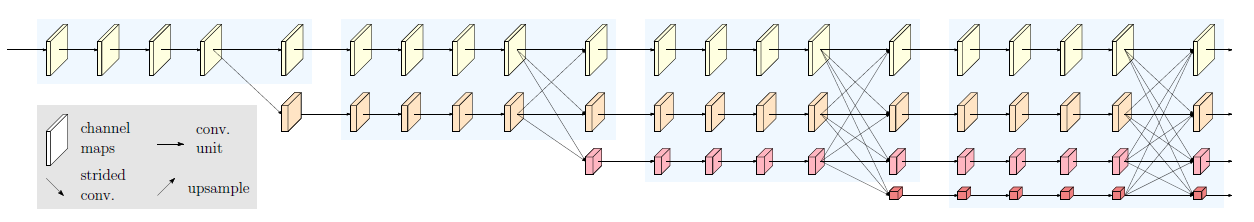
\includegraphics[width=0.8\linewidth]{2.png}
   \end{center}
      \caption{Structure of HRnet from the paper}
   \label{fig:long}
   \label{fig:onecol}
\end{figure}

From the figure we can tell that there are two modules in this model,
parallel multi-resolution convolution and repeated multi-resolution fusion.
Therefore, we would like to introduce those modules and some our difference.

One key improvement of HRnet is the parallel the convolution stream in previous models.
Each line of convolutions is a paralleled stream of certain resolution.
In HRnet, each resolution is assigned to a stream of convolutions
and these streams are processed together.
Blocks in each stream are basic blocks in ResNet.
When initializing each stream,
there is a multi-resolution fusion module to exchange information from different resolution convolution streams to reduce information loss.
Specific formulas of each module is illustrated in the paper explicitly.
We will not list the formulas here.

Moreover, we found a problem while reading the source code.
From the structure we can tell that
in each multi-resolution fusion module,
the initialed stream gains the information from all previous convolution streams.
However, in the source code,
The initialed stream only accept the information of the convolution with the lowest resolution in previous streams.
In our reproduced model, we applied the structure in the paper.
The improvement in performance is negligible,
but there's indeed difference.

\section{Technique Details}

We use Python language with PyTorch framework.
As mentioned, our model is structured different from the source code.
To emphasize the difference,
we made a figure to show our structure:

\begin{figure}[h]
   \begin{center}
      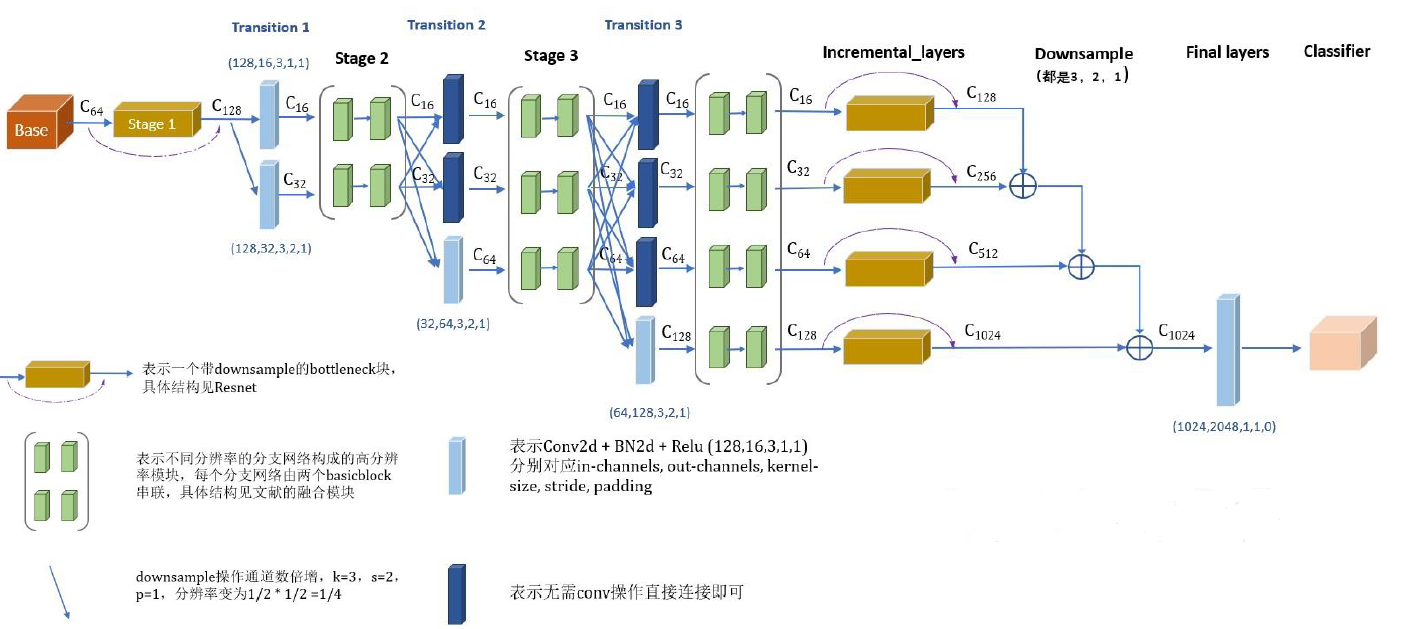
\includegraphics[width=0.8\linewidth]{3.png}
   \end{center}
      \caption{Our structure.}
   \label{fig:long}
   \label{fig:onecol}
\end{figure}

This is a simplified but more explicit representation of the structure.
We built our model based on it.

\section{Experiments and Performance}

Our experiment settings are listed here.

\begin{table}[h]
   \begin{center}
   \begin{tabular}{|c|c| p{5cm}|}  
   \hline  
   Batch size & 32 \\
   \hline  
   Optimizer & SGD \\
   \hline  
   Scheduler & CosineAnnealing \\  
   \hline
   Learning rate & 1e-3 \\
   \hline
   \end{tabular}  
   \end{center}  
\end{table}

The reproduced model and the initial model in the paper both share these settings.
We ran the experiment for 100 epochs until the loss curve converged.
The running time for each epoch is around \emph{to do}.
Here's the performance of the two models:

\begin{figure}[h]
   \begin{center}
      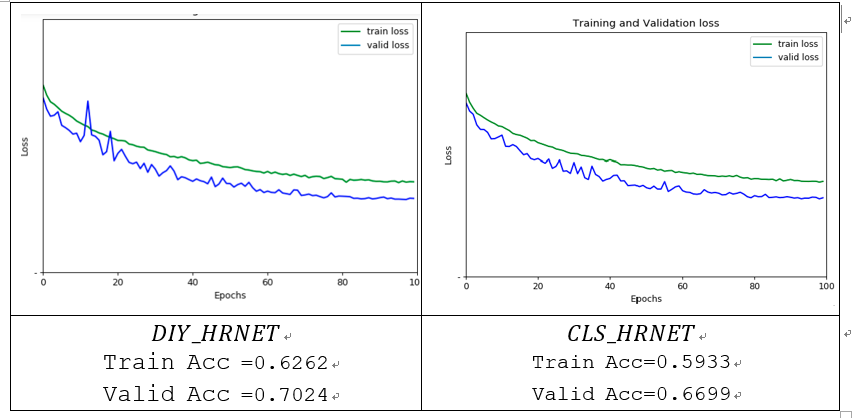
\includegraphics[width=0.8\linewidth]{1.png}
   \end{center}
      \caption{The performance of two models. The left one is our model 
      and the right one is scratched from the paper.}
   \label{fig:long}
   \label{fig:onecol}
\end{figure}

The trend of loss and accuracy is similar.
And after 100 epochs, the performance of our model is better than the initial model.

\section{Insights Analysis}



\section{Conclusion}

HRnet is the state-of-art model in high-resolution representation field.
It entirely reshaped the structure of previous model,
importing parallel streams and fusions.
As mentioned in the class,
breakthroughs in the deep learning is not refining the current models
or applying current models in other fields.
Only innovation like this can lead to the improvement in the entire field.

Also, by digging into a paper and its source code,
we found the details behind the paper.
While reading papers,
we always just go through the context and comprehend the model easily.
That's far from enough.
Only by burying ourselves in the paper can we understand the paper thoroughly.

{\small
\bibliographystyle{ieee_fullname}
\bibliography{egbib}
}

\end{document}
